\documentclass[10pt, letterpaper, openany]{book}
	\usepackage{graphicx}
	\usepackage{natbib}
	\usepackage[margin=.7in, paperwidth=6in, paperheight=9in]{geometry}
	\usepackage{longtable}
	\usepackage{pdfpages}
	\usepackage{pifont}
	\usepackage{enumitem}
	\usepackage{array}
	\usepackage{setspace}
	\usepackage{titlesec}
		\titleformat{\chapter}{\normalfont\huge}{\thechapter.}{16pt}{\huge\bf}
		\titlespacing{\section}{0pt}{*2}{*0}
		\titlespacing{\chapter}{0pt}{*-3}{*3}
		\titlespacing{\subsection}{0pt}{*0}{*0}
		\titlespacing{\subsubsection}{0pt}{*0}{*0}
		\renewcommand{\chaptername}{}
	\usepackage{enumitem}
		\setlist{itemsep=.5pt}
	\setlength{\parskip}{1em}

\title{
\includegraphics[scale=0.35]{../../../img/logo.png}\\Applied Rationality Handbook}
\author{Berkeley 2016}
\date{}
\pagestyle{headings}

\begin{document}
	\maketitle
	\clearpage
\chapter*{How to use this book}
Welcome, participant!

This is your content handbook.  It's meant as a reference material, so that you can examine the theoretical underpinnings of our techniques, refresh yourself on particular steps or methods, and go beyond what's taught at the workshop.  Each technique has its own section, including:

\begin{itemize}
\item \textbf{Epistemic status} --- This is a measure of how closely linked to established cognitive science research a given technique is (versus those we have discovered through practical iteration, but not yet gathered formal data on).
\item \textbf{Step-by-step breakdown} --- While we encourage participants to mix, match, refactor, and tinker, we've distilled our basic algorithms into their most useful forms.
\item \textbf{Common mistakes and FAQ}
\item \textbf{Resources for further exploration}

While you may be tempted to read ahead, be forewarned---we've often found that participants not only have an easier time understanding our content if they hear it first, but also have a \emph{harder} time grasping it if they've already tried to put it together from the text.  Many of the explanations are intentionally approximate or incomplete, and most of them rely on terminology and context that's best transmitted in person.  It helps to think of this handbook as a companion to the workshop, rather than as a standalone resource.

\textbf{You do \emph{not} need this handbook during our classes;} your workbook contains all of the information and prompts you will need for our lectures and activities.  That being said, we hope that, between classes and after the workshop, this handbook provides you with lots of food for thought.  Don't be afraid to scribble notes in the margins and jot down your own annotations, and let us know if you find yourself discovering connections we haven't thought of!
\clearpage




	\tableofcontents
	\part*{Introduction}
		\addcontentsline{toc}{part}{Introduction}	
		\clearpage
			\addcontentsline{toc}{chapter}{What is ``Applied Rationality''?}
				\chapter*{What is ``Applied Rationality''?}
	
	\section*{Aiming to answer the right questions \ldots}
	Imagine that an intelligent, curious person meets with you for lunch, and begins asking you about your field of expertise.  At first, you talk mainly about your own day-to-day work, but eventually the conversation turns to the big, open questions---what are the most important unsolved problems in your profession?  Why do they matter?  What kinds of things change once you and your colleagues break through?  After you share your perspective, your new acquaintance nods thoughtfully, and asks one final question:
	
	``So, why aren't you working directly on \emph{that}?"
	
	There's a useful (and somewhat friendlier) generalization of this way of thinking.  At any given time in our lives, it's possible (though not always easy!) to answer the question, ``What is the \emph{most} important problem here, and what are the things that are keeping me from working on it?"  We refer to this as ``asking the Hamming question," as a nod to mathematician Richard Hamming, who was notorious for doing the above with his colleagues at Bell Laboratories.
	\\
	\section*{\ldots while accounting for cognitive imperfections.}
	When we make decisions and analyze information, we tend to move back and forth between two broad kinds of thought---one faster, more automatic, and more closely tied to our emotions, and the other slower, more effortful, and more closely tied with our explicit thoughts and beliefs.  In his book \emph{Thinking Fast and Slow}, Nobel Prize winner Daniel Kahneman described them as \textbf{System 1} and  \textbf{System 2}:
	
	\renewcommand{\arraystretch}{1.2}
		\begin{table} \small \centering
			\begin{tabular}{ |c|c| }
			\hline
			\textbf{System 1} &  \textbf{System 2} \\
			\hline \hline
			 Evolved earlier & Evolved later, more unique to humans \\
			 Wordless, ``black box'' thinking & Verbal, ``transparent" thinking \\
			 Processes information quickly & Processes information slowly \\
			 ``Intuition,'' ``reflex,'' etc. & ``Concentration,'' ``reflection,'' etc. \\
			 Always on & Often on standby \\
			 Doesn't use working memory & Limited by working memory \\
			 \hline
			 \end{tabular}
		\end{table}
	 
	 Each ``system'' is complex, made up of a variety of parts, and neither is perfect.  Our knee-jerk, automatic processes are prone to making the wrong connections---if a new acquaintance resembles an old enemy, you may find yourself feeling anxious or cold without really knowing why.  Our deliberate, explicit processes can fail by leaving out information---if you can't put a fleeting feeling of unease into words, you may be tempted to disregard it, and exclude it from your calculations.
	 
	 Often, people make the mistake of thinking that rationality is the process of muting those primitive, intuitive processes and just relying on System 2.  It's an understandable mistake---after all, those are the ``higher brain'' functions, the ones that allow us to do things animals can't, like writing and philosophy and math and science.
	 
	 But turning off or ignoring large parts of your brain is rarely helpful, and applied rationality is about using \emph{every} tool in your possession.  In the classes at this workshop, we'll talk about how to balance and combine these two types of thinking, learning to understand the strengths of each so that you know when to bring them to bear and how to use them effectively both together and apart.  The aim is to make deliberate, thoughtful use of your \emph{whole} mind---a whole that's much greater than the sum of its parts.

\begin{center}

\includegraphics[width=\textwidth]{../../../img/lineshalf.png}
\end{center}		
		\chapter*{Advice from Opening Session}
			\addcontentsline{toc}{chapter}{Advice from Opening Session}
			\section*{Make good quiche}

Imagine that you have a friend who is creating a recipe book.  You've agreed to help your friend beta test some of their recipes, and they've handed you a rough draft of instructions on how to make quiche.

As you're reading through the recipe, you begin to notice a few ... let's say, \emph{problematic} steps.  For instance, the recipe calls for six ``whole eggs,'' which to you seems to imply shells and all.  It also says to bake for 4.5 hours at 450 degrees, and calls for 10 tablespoons of salt.

Now, one way that you might offer productive feedback to your friend is to follow the recipe \emph{exactly as written,} creating a crunchy, salty, burned quiche.  This is actually a pretty helpful strategy, early on---it's a way to stress-test the recipe to see exactly how broken it is.

However, if you \emph{also happen to want some quiche}, there's another method you might employ.  Instead of following steps that are obviously wrong, you could instead \emph{try to make good quiche}, treating the recipe as more of an inspiration than a strict set of instructions.  You could throw away the eggshells, drop the time and temperature down to (say) 45 minutes at 350 degrees, and throw in just a pinch of salt.  Maybe you'll even have some additions that your friend didn't think of, like mixing in some chopped kale.

At the end of \emph{that} process, you'll not only have notes about flaws in the original recipe, but also constructive suggestions and---most importantly---a delicious meal you can actually eat.  You'll have something that's useful to \emph{you}, both in the moment and for the future.

Like your friend's quiche recipe, many of the concepts and techniques within the workshop are experimental.  There will be times when they seem a little off, and other times when they may seem clearly false.  It helps to remember that the goal is not to improve our recipe book, but to \textbf{make good quiche}.  That means that, instead of doing things that don't make sense, you should feel free to tinker, experiment, and modify.  Your perspective is unique---while we have a lot of insight to offer, there's no one who better understands your own life and mind than you.  If we seem to be pointing in the wrong direction, feel free to head in the right one, instead---and afterward, let us know what you discovered.
			\clearpage
\section*{Boggle!}

There's a way in which education tends to make knowledge very \emph{flat}.

Let's take the Earth and the Sun, for example.  If I were to ask you about the relationship between the two, you'd probably offer me the well-worn phrase ``the Earth revolves around the Sun.''  It's automatic, reflexive, almost atomic---once you start with ``the Earth,'' you barely have to think anymore.  The ``revolves around the Sun'' part just fills itself in.

But once upon a time, people didn't \emph{know} that the Earth revolved around the Sun.  In fact, people didn't even really know what the Earth and the Sun \emph{were}---they thought they did, but looks can be deceiving.  It took us multiple geniuses and the innovations of centuries to go from ``the Earth is a flat plane and the Sun travels across the celestial sphere'' to the factoid that we repeat back to our teachers in a bored monotone.  Somehow, all of the confusion and excitement of discovering that the Sun is an incandescent ball of hydrogen and that the Earth is tied to it by the same fundamental force which makes pendulums swing and that both of them are round except \emph{not quite} and that gravitational attraction is proportional to the square of the distance except \emph{not quite}, don't forget relativity and quantum mechanics and---

---somehow, all of that gets lost when we flatten things out into ``the Earth revolves around the Sun.''

Fortunately, there's a solution---\emph{boggling.}  You're reading a book!  What's a book?  I mean, okay, it's just a book.  But what is it \emph{really?}  I mean, where did these pages come from?  Who wrote them?  Who manufactured them?  How could \emph{you} make a book?  I mean, maybe you've already made one.  But how did the paper get made?  And what's printer ink made of, anyway?  And where did the ideas come from?  And language!  These squiggles on a page carry \emph{meaning!}  How'd we come up with that?  What's actually going on in your brain, when you look at these squiggles and find yourself thinking thoughts?  What even \emph{is} a thought?  I hear there are neurons involved---how does \emph{that} work?

When you allow yourself to embrace confusion, and turn away from the cached, easy, empty answers, you start to see a much richer, deeper world, with many more opportunities to learn and to grow.  During the workshop, there will be many things that \emph{seem like} stuff that you already know, just as you already know that the Earth revolves around the Sun.  But don't be fooled!  Surface explanations are the opposite of knowledge---they're a curiosity-killer, preventing you from noticing that there's stuff you still don't \emph{get}.  Human cognition is one of the most complex, opaque, and difficult phenomena we've ever encountered.  As you study it, don't settle for flat knowledge---instead, \emph{boggle.}
			\clearpage
\section*{Try Things!}

When you're considering adopting new habits or ideas, there's no better way to gather data than \emph{actually trying.}  It's often faster and simpler to just give things a shot and see how it goes than to spend a lot of time trying to anticipate and predict whether or not you'll find something worthwhile.

This is particularly important because when something \emph{does} work out, \emph{you get to keep doing it.}  If your friends have recommended five different activities to you, and you've only liked one of them, it's easy to think of the whole process as a pretty big waste of time:

\setlist[description]{leftmargin=6cm,labelindent=6cm}
\begin{description}
	\item[\ding{55}] Yoga
	\item[\ding{55}] Ultimate Frisbee
	\item[\ding{55}] Dungeons \& Dragons
	\item[\ding{52}] Meditation
	\item[\ding{55}] Salsa dancing
\end{description}

An 80\% failure rate isn't exactly encouraging, after all.  But what the above framing fails to take into account is the magnitude of even a single success.  Instead of four bad experiences and one good one, what's \emph{actually} going on is more like the following:

\begin{center}
  \begin{tabular}{ | l | c | c | c | c | c | c | c | c | c |}
    \hline
    Activity & T1 & T2 & T3 & T4 & T5 & T6 & T7 & T8 & T9 \\ \hline
    Yoga & \ding{55} & \ding{55} & & & & & & & \\ \hline
    Ultimate Frisbee & \ding{55} & & & & & & & &  \\ \hline
    Dungeons \& Dragons & \ding{55} & \ding{55} & \ding{55} & & & & & &  \\ \hline
    Meditation & \ding{52} & \ding{52} & \ding{52} & \ding{52} & \ding{52} & \ding{52} & \ding{52} & \ding{52} & \ding{52} \\ \hline
    Salsa dancing & \ding{55}  & & & & & & & & \\ \hline
    \end{tabular}
\end{center}

When you look at it this way, you can see that the failed trials are more than compensated for by the sustained run of a now-successful habit.  Indeed, when it comes to hobbies and activities that might last you the rest of your life, it becomes worthwhile to establish a habit of trying things that have even a one-in-ten or one-in-a-hundred chance of being enjoyable.  It only takes a few paying off to make the whole thing worthwhile.

So while you're listening and participating this weekend, be on the lookout for opportunities to turn our lessons into actions that you can try out.  Translating class material into practical experiments is a great way to digest material anyway, and it'll help you decide which techniques are most worth prioritizing when you return home.
			\clearpage
\section*{Be Present}

One key element of getting the most out of an experience is being \emph{present}. This includes physically showing up, but it also includes having your mind in the room and your background thoughts focused on the content. The more you're taking calls and answering texts and keeping up with social media and what's going on back home, the more you'll remain in your ordinary mental space, continuing to reinforce the same habits and patterns you're here to change.  There's a sort of snowball effect, where even a little disengagement can make absorbing the value you'd like from a workshop rather difficult, which confirms a suspicion that there's no value to be had, and so on.

In addition to external distraction, we've also found that there are a few unhelpful narratives that participants occasionally find themselves repeating---narratives which make it hard to engage with the content and block opportunities for asking good questions and taking new steps.  If you notice one of these narratives cropping up in the back of your mind, we encourage you to try deliberately setting it aside, as an experiment---let it go, see what happens, and judge for yourself.  Our staff are happy to chat with you about any of these, if you think you might find that helpful.

\begin{itemize}
	\item \textbf{``I'm too dumb/old/lazy to learn this."} We sometimes encounter people who think that, because they don't measure up to some standard or another, they aren't ``good enough'' to benefit from the workshop material.  As a counter to this, we recommend donning a \emph{growth mindset}: if it can be learned by a human, it can be learned by you.	
	\item \textbf{``I already know this part."} Some people come into our workshop with significant background knowledge and, when they start to see familiar material, slip into a mode of assuming there's nothing for them to learn.  Unfortunately, this can mean that you're ``turning off'' right at the moment that we're offering new insight.  To counter this, we recommend that you try to approach \emph{every} class with fresh eyes.  Even if the core concepts are familiar, look for the fine detail---the places where your peers and instructors have made valuable connections you might have missed.  In particular, try to be interested rather than interesting---there's more to gain from stealing new insights than rehashing thoughts you've already thought.
	\item \textbf{``I've got important things to do, and this lesson can wait."} Sometimes there really \emph{are} important things to attend to. But if they're on your mind during the workshop, you're likely to have a hard time absorbing the material in a way that will stick. We recommend that you set aside what you can, and \emph{fully address} what you can't set aside: if something really can't wait, step out, make it your sole focus until it's dealt with, and return with full and fresh attention.
\end{itemize}

	\part*{Core Classes}
	\clearpage
		\addcontentsline{toc}{part}{Core Classes}
			\addcontentsline{toc}{chapter}{Inner Simulator}
			\setlength{\parindent}{0em}
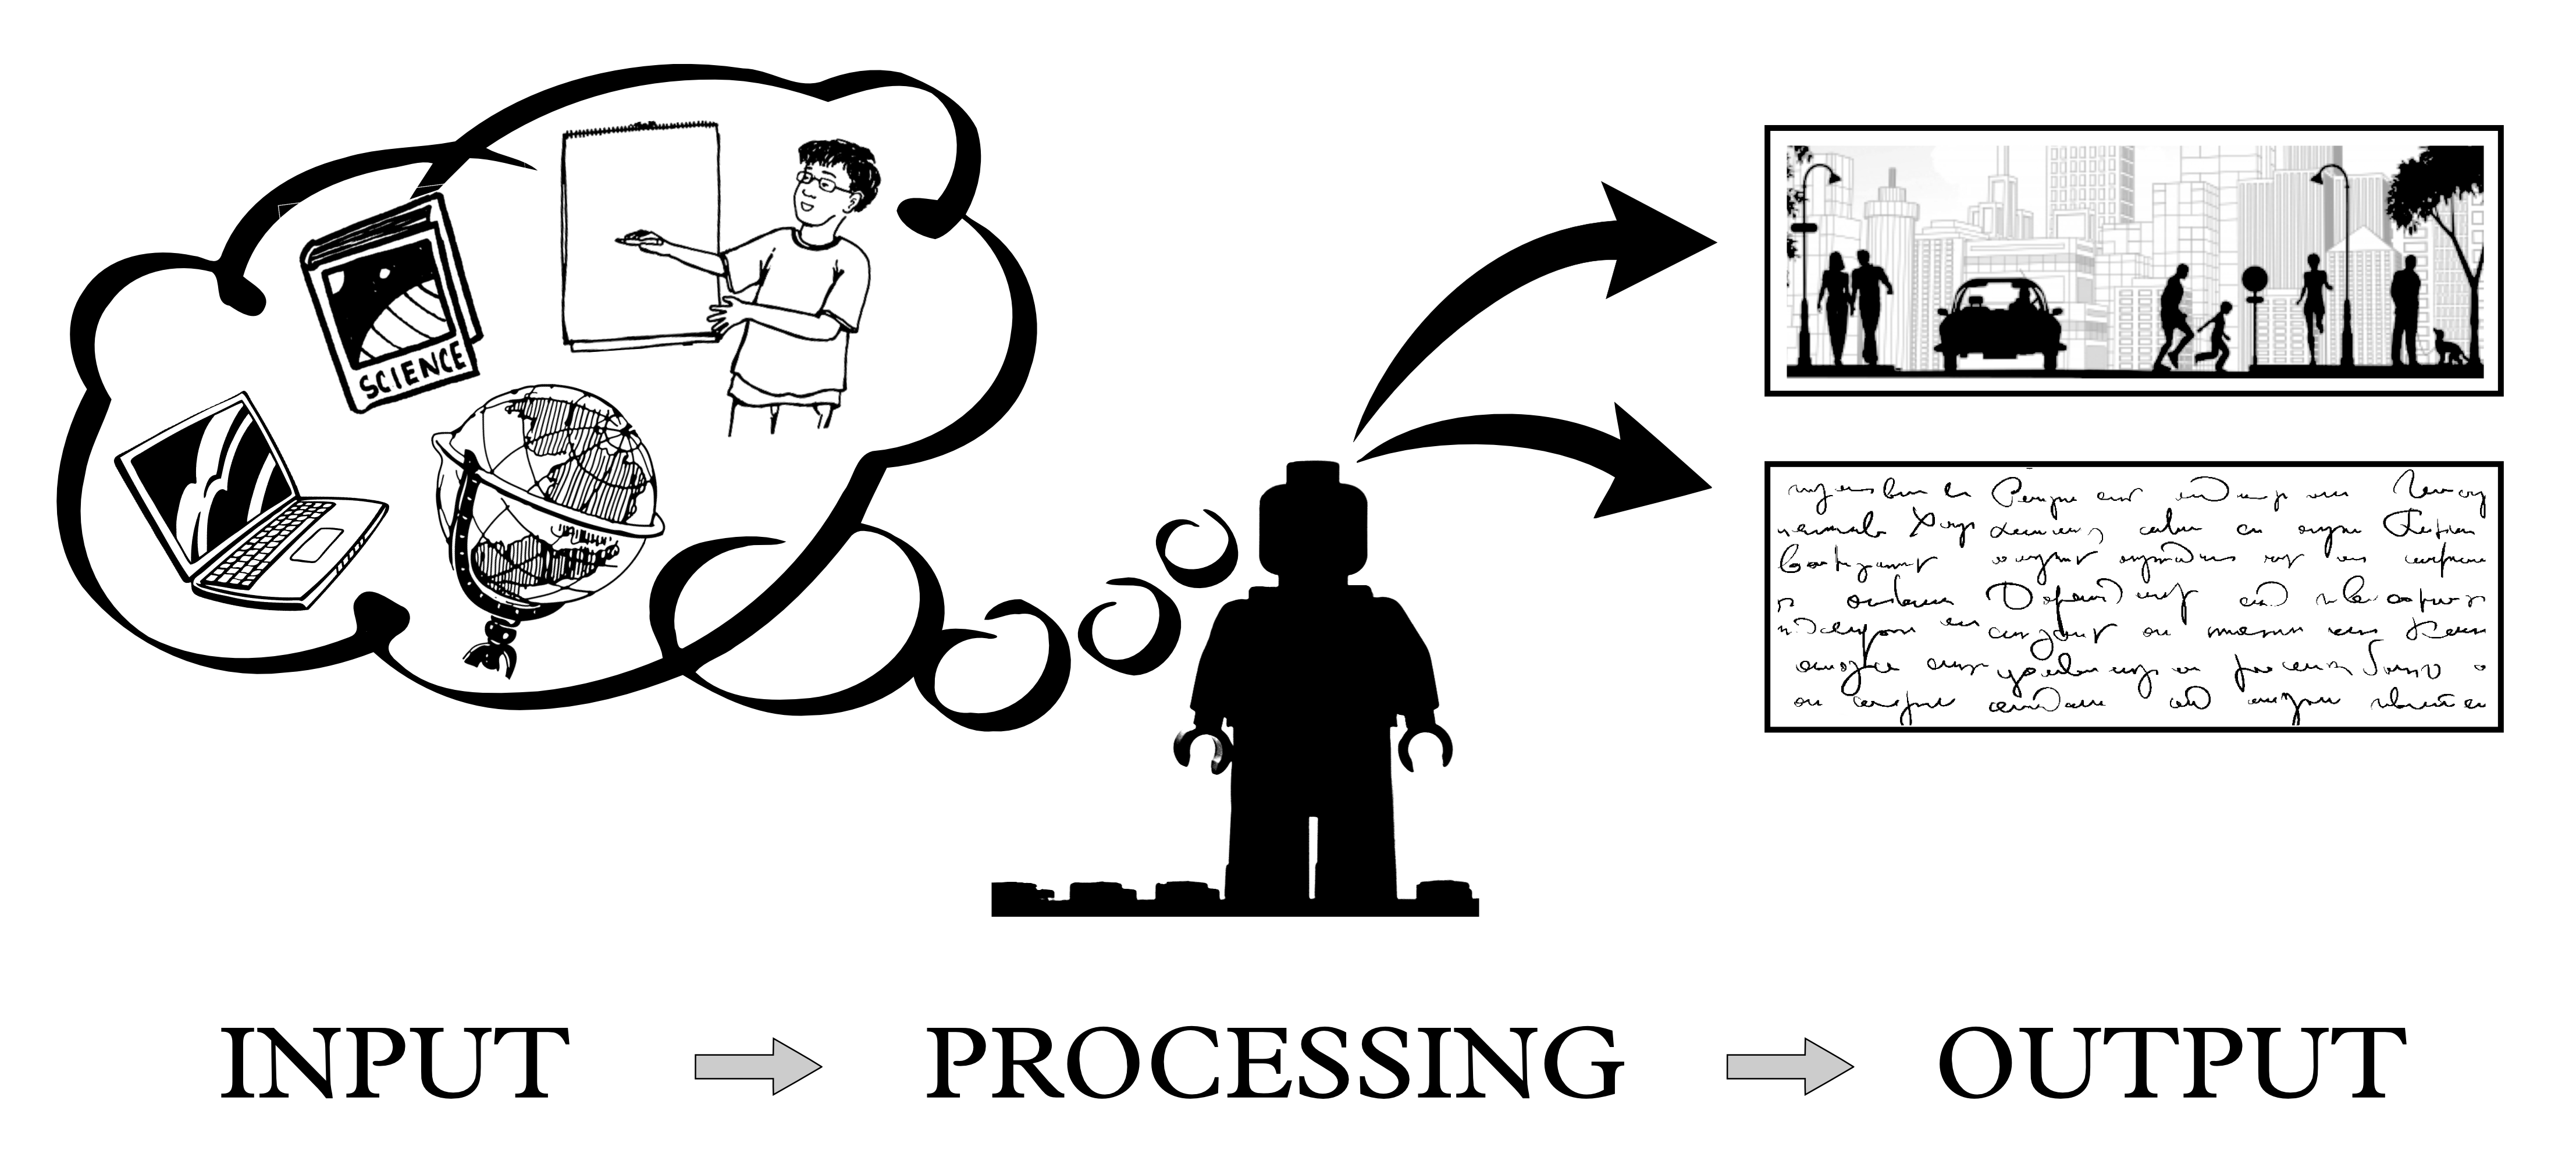
\includegraphics[width=\textwidth]{../../../img/innersim.png}

When you move to catch a falling pen, or notice that your friend is upset just by the way they entered the room, you're using your \textbf{inner simulator}.
\begin{center}
	\begin{tabular}{ | p{.5\textwidth} | p{.5\textwidth} | }
		\hline
		\textbf{Inner Simulator} & \textbf{Explicit/Verbal Models} \\ \hline
		Intuitive; part of System 1 & Analytical; part of System 2 \\ \hline
		Outputs feelings, urges, reflexes, and vivid predictions (sometimes called ``anticipations'') & Outputs arguments, calculations, and explicit models (sometimes called ``professions'') \\ \hline
		Learns well from experience and examples and responds to being \emph{shown} & Learns well from textbooks, statistics, Wikipedia, etc. and responds to being \emph{told} \\ \hline
		Good at social judgment, routine tasks, and any situation where you have lots of experience & Good at comparisons and reframings (e.g. noticing that \$1/day $\approx$ \$350/year) \\ \hline
		Powerful generator of narratives and explanations, but vulnerable to framing and subconscious question substitution & Powerful generator of plans and models, but vulnerable to distortion from wishful thinking and ideology \\ \hline
	 \end{tabular}
 \end{center}

\setlength{\parindent}{1.5em}
Each of us carries around a rich, complex model of the universe in our head, assembled from a lifetime of experiences and memories.  We don't have to \emph{think} about how to catch a falling pen, because our inner simulator \emph{knows} how falling objects move.  Similarly, it knows what facial expressions mean, what it's like to drive from home to work, and what sorts of things \emph{tend to go wrong} given a set of circumstances.  It's a powerful tool, and learning how to access it and when to trust it is one of the first steps to becoming a whole-brain thinker.

\section*{Prompts for your inner sim}
\setlength{\parindent}{0em}
Not every problem is appropriately addressed with your inner sim---you can imagine it as a single piece of hardware with a few built-in functions.  It's very, very good at doing those functions, and not so great with most other things (for instance, inner sim is terrible at understanding large numbers, and causes us to donate \emph{the same amount of money} to save 8,000 or 800,000 hypothetical birds from oil spills).  Here are three types of question your inner sim \emph{is} good at answering:

\subsubsection{What happens next?}
Start a ``mental movie'' by concretely visualizing a situation, and see what your brain \emph{expects to happen.}  Given the following inputs, what would be the output?
\begin{itemize}
	\item \textbf{Input:} A laptop is balanced half-off, half-on the edge of a table in a crowded, busy office.
	\item \textbf{Input:} You lift a piece of watermelon to your mouth and take a bite.
	\item \textbf{Input:} You sneak up on a friend at work, take aim with your water gun, and pull the trigger.
\end{itemize}

\subsubsection{How shocked am I?}
Check your ``surprise-o-meter''---visualize a scenario from start to finish, and see whether you ``buy'' that things would actually play out that way.
\begin{itemize}
	\item \textbf{Input:} You've purchased food for a 25-person party, and 20 people show up.
	\item \textbf{Input:} Same party, but \emph{70} people show up.
	\item \textbf{Input:} You finish your current project in less than half the time you allotted for it.
\end{itemize}

\subsubsection{What went right/wrong?}
Use your ``pre-hindsight''---start by assuming that your current plan has utterly failed (or gone extremely well, but that's the side we're already biased toward believing).  What explanation leaps to mind about why this happened?
\begin{itemize}
	\item \textbf{Input:} Think of a \emph{specific} email you intend to send in the next few days.  Turns out, the person you sent it to was extremely irritated by it.
	\item \textbf{Input:} Imagine you receive a message from yourself from the future, telling you that you should \emph{absolutely} stay at your current job, and keep up the good work.
	\item \textbf{Input:} It's now been three months since your CFAR workshop, and you have yet to make deliberate use of your inner simulator.
\end{itemize}
\clearpage

\section*{Being specific: Making good use of your inner simulator}
Like most algorithms, your inner simulator will output good and useful information if you give it good and useful input, and it will output useless garbage if that's what you feed it.  It's an especially good check on wishful thinking and motivated cognition---just imagine its response to a list of New Year's resolutions---but you need to make sure that you aren't rigging the game by phrasing questions the wrong way.

\setlength{\parindent}{1.5em}
Two useful strategies for avoiding vague, open-ended ``garbage'' are sticking to \emph{concrete examples} and looking for \emph{next actions}.

\subsubsection{Asking for Examples}
\newenvironment{blockquote}{%
  \par%
  \medskip
  \leftskip=4em\rightskip=2em%
  \noindent\ignorespaces}{%
  \par\medskip}
\begin{blockquote}
``It's just so \emph{frustrating.}  It's like, every little thing turns into a fight, you know?  And then it's \emph{my} fault that we're fighting, and I have to either pick between defending myself or smoothing things over, and since I'm the only one who ever wants to smooth things over, that means that I'm always the one apologizing.  And last week---I told you about what happened while we were stuck in traffic, right?  No?  So, like, out of \emph{nowhere,} while I'm trying to focus on not getting into a wreck, all of a sudden we're back talking about grad school \emph{again}\ldots''
\end{blockquote}

In a situation like this, your inner sim has nothing to grab onto---everything is vague, everything is open to interpretation, and clich\'es and stereotypes are filling in for actual understanding.  It could be that your friend is in the right, and needs your commiseration; it could be that the situation calls for some harsh truths and tough love.  How can you tell, one way or another?  Try some of these:
\begin{itemize}
	\item{What were the last couple of things you fought about?}
	\item{What were you talking about right before grad school came up?}
	\item{When you say you're the only one who wants to smooth things over, what do you mean?  What are you seeing and hearing that give you that sense?}
\end{itemize}

When it's just ``every little thing turns into a fight,'' your inner sim literally doesn't know what to think---there are too many possibilities.  But when the argument started with ``Do we really have to go over to Frank's \emph{again?}'' or with ``Oh, hey, I see you got new shoes.  Nice!'' you have a much better clearer sense of what the situation really looks like.

Asking for examples is a handy technique for any conversation.  When you keep your inner simulator engaged, and keep feeding it data, you might notice that it's easier to:


So, those are three common and useful function calls, but don't forget---the algorithm is only as good as the input it is given.  Your inner simulator is especially good at being a check on wishful thinking or what you feel like you \emph{ought} to believe---picture its response to a list of New Year's Resolutions---but you need to make sure that your explicit/verbal models aren't rigging the game by phrasing questions the wrong way.  If you pass your inner simulator vague, open-ended input, it will happily give you 
























Being Specific: Making the Best Use of Your Inner Simulator 

These are three ways you can make function calls on your Inner Simulator, but how can you make sure you?re passing it the best inputs?  Your Inner Simulator is especially good at being a check on wishful thinking or what you feel like you ought to believe, but you need to make sure your explicit/verbal models aren?t rigging the game by phrasing questions the wrong way.  

By being specific, concrete, and vivid, you can mostly avoid getting stuck in Garbage In, Garbage Out.  Using concrete examples and next actions will help.

Ask for Examples!
For a concrete example of using examples, try this story from Surely You?re Joking, Mr. Feynman!
I had a scheme, which I still use today when somebody is explaining something that I'm trying to understand: I keep making up examples. For instance, the mathematicians would come in with a terrific theorem, and they're all excited. As they're telling me the conditions of the theorem, I construct something which fits all the conditions. You know, you have a set (one ball) - disjoint (two balls). Then the balls turn colors, grow hairs, or whatever, in my head as they put more conditions on. Finally they state the theorem, which is some dumb thing about the ball which isn't true for my hairy green ball thing, so I say, "False!"
If it's true, they get all excited, and I let them go on for a while.  Then I point out my counterexample.  
"Oh.  We forgot to tell you that it's Class 2 Hausdorff homomorphic."
Your inner simulator needs something to visualize.  Just saying something as words isn?t enough.  You want something specific that your imagination can interact with.  You can ask yourself for examples, too!

Asking for examples is a really handy thing to do in conversation.  When you keep your Inner Simulator engaged during a conversation, and keep feeding it data, you might notice that it?s easier to:
1. Notice if your friend?s claim is false ? Just like Feynman, you may be able to notice where the error is, instead of just having a vague sense of something not adding up if you?re concrete.
2. Notice if you?re misunderstanding your friend ? When we listen to someone else, we try to approximate and anticipate what they?re explaining.  If you ask for examples from your friend, you can see if you?ve been accidentally adding or leaving out extraneous features on yours.
3. Notice if you?re the one who?s wrong ? It?s easy to avoid noticing if you?ve made a mistake; it?s painful!  The more concrete your disagreement is, the easier it is to notice if there?s a flaw in your own argument and to own up to it.

Next Actions

A goal isn?t the same thing as a plan.  I might have the goal of exercising more, but to have a plan I need to think about when I?ll go to the gym, what I?ll do, and how I?ll remember in the moment.  

But before I get up to any of those parts of the plan, I?ll need to take my next action, which might be printing out my gym coupon or setting a reminder in my calendar or choosing a time to go buy workout clothes.  A next action is the step that sets your plan in motion.  It?s the first thing you?d have to do to keep the plan going, which is often as pedestrian as putting something on your calendar or placing a library hold or asking someone to have coffee to talk over the plan.  Often, when you?re deciding on a next action, it?s helpful to think about a trigger ? some specific event or time that reminds you to do your next action (such as 5pm Tuesday, or when my boss returns my email, or when I wake up tomorrow morning )

Write down one goal you have (a larger scale thing you want to accomplish):
Take a few minutes to think about your plan to make this goal happen.  What?s the next action you need to take to get the plan moving?
What specific trigger will let you know when it?s time to complete this next action?
Now practice going through this process a few more times: 
Goal:
Next action: 
Trigger: 
Goal: 
Next action: 
Trigger:
Inner Simulator Practice: Murphyjitsu!

Murphy?s Law says that anything that can go wrong will go wrong, but you can use some of the skills and safeguards you?ve learned for your Inner Simulator to anticipate and evade these hazards.
Step 1: Pick a plan/project/goal
Step 2: Make it specific enough to visualize. 
What?s the next action you would need to take to keep this project/plan moving forward?  It should be concrete enough that you can picture yourself doing it, not something vague like ?work out more.?
Step 3: Check your surprise-o-meter
Visualize putting this plan in motion, then ask, how surprised would I be if this plan failed?  If you?d be shocked, then you?re done!  Otherwise, continue to step 4.
Step 4: Use Pre-Hindsight
Your plan didn?t work!  And it failed at the stage of the next action you wrote in Step 2!  What happened?
Step 5: Use Looking Forward
What action would you have had to take to prevent this particular failure mode?  Visualize taking this preemptive action and then ask ?What comes next??  Have you successfully defused the danger?  Did you create a new weak point to patch?
Step 6: Iterate!
Repeat Steps 3-5 several times (sometimes this technique is called ?Simulate 17 times, act once?).  What else might have gone wrong?  What could have prevented it?  You?re battle-hardening your plan against happenstance and poor habits.  Remember that this should be very quick ? all ?17? iterations should take maybe a few minutes total.

	\part*{Flash Classes}
		\addcontentsline{toc}{part}{Flash Classes}
	\part*{Additional Resources}
		\addcontentsline{toc}{part}{Additional Resources}
		\chapter*{Glossary}
			\addcontentsline{toc}{chapter}{Glossary}
			\clearpage
\begin{longtable} { p{.3\textwidth} p{.7\textwidth} }

\textbf{80-20} & To ``80-20'' something is to obtain most of the result (80\%) with only a small proportion of the work (20\%).  This expression originates with the Pareto principle which states that for many events, 80\% of the effects come from 20\% of the causes (e.g. most of a company's sales come from a small number of its clients).\\

\textbf{Affect} & One's emotional state or disposition, especially as evidenced by one's body language, facial expression, word choice, and tone of voice.\\

\textbf{Affordance} & An opportunity or potential-for-action arising from a given context; a door handle creates an \emph{affordance} for pulling.  In particular, it is a \emph{genuine} or \emph{felt} opportunity---while there may be no physical difference between picking up a pen on one's own desk, one's coworker's desk, one's manager's desk, or the CEO's desk, each of those contexts provides a different degree of affordance.\\

\textbf{Againstness} & The quality of resistance to information, often caused by strong emotion or sympathetic nervous system activation, but also resulting from conflicts with one's identity, inherent biases, and other entangled beliefs.\\

\textbf{Agency} & The property of both having and exercising a capacity for relevant action; one's ability to meaningfully affect the world around oneself and effectively move toward achieving one's goals.  In particular, agency implies the ability to move beyond default patterns and cached answers, and to think and act strategically.\\

\textbf{Alief} & See ``anticipation.''\\

\textbf{Anticipation} & A deeply-felt belief, sometimes called an ``alief,'' emerging naturally from one's mental model of the universe.  Sometimes contradictory to one's \emph{professions}, which are explicitly stated beliefs---for instance, one might profess/believe that a high wooden bridge over a canyon is entirely safe, and yet reveal an anticipation/alief of danger by tensing, moving gingerly, and refusing to look down.\\

\textbf{Aumanning} & From Aumann's agreement theorem, which demonstrates that two rational agents with the same background beliefs cannot disagree.  Aumanning refers to one of several processes (such as double crux) for resolving disagreement by converging on a shared model of reality.\\

\textbf{Aversion} & An internal repulsion or desire-to-avoid, sometimes referred to as a ``yuck factor'' or ``ugh field.''  Aversions may have clearly identifiable sources and mechanisms (e.g. aversion to exercise related to feelings of heat, sweatiness, pain, or exhaustion), or they may be difficult to pin down.  Typically, aversions either cause one to spend less time and energy interacting with a person/task/activity, or color those interactions with pain or stress.\\

\textbf{Aversion Factoring} & A technique for addressing aversions by first zeroing in on their concrete, immediate sources and then evaluating each aversion for validity or relevance and taking steps accordingly.\\

\textbf{Bayesian Updating} & A method of shifting belief in response to new evidence, derived from Bayes' Theorem in statistics.  Formal Bayesian updating requires use of a mathematical formula, but a rough, approximate version involves stating an explicit belief with a given probability (a ``prior''), evaluating the degree to which new evidence bears upon that belief, and making an incremental adjustment to one's evaluation of its likelihood in response, resulting in a ``posterior'' that is meaningfully different.\\

\textbf{Bias} & A systematic distortion of one's actions or reasoning due to factors not relevant to the situation at hand (e.g. one might reject a new policy recommendation out of a ``status quo bias,'' in which one favors current ways of doing things regardless of cost or opportunity).\\

\textbf{Black Swan} & A rare and essentially unpredictable event with significant negative consequences.  Classic examples of black swans include things like meteor strikes, the 9/11 terrorist attacks, the sinking of the Titanic, and the arrival of Europeans in the New World (from the perspective of the indigenous populations).  The term is also used metaphorically, to refer to events with disproportionate and unexpected personal or small-group impact.\\

\textbf{Blindsight} & Classically, an effect whereby individuals with certain types of blindness can nevertheless ``see'' in the sense that their unconscious mind is processing information that they are not consciously aware of.  These individuals can correctly identify the position of lit dots on a black screen by ``guessing,'' at a rate far higher than chance would allow.  Metaphorically, blindsight is used to refer to instinctive or visceral knowledge that tends to be more correct than one would expect, thanks to accurate processing by one's subconscious processes.\\

\textbf{Boggle!} & An imperative reminder to embrace confusion and seek deeper understanding.  One is more likely to learn and grow if one \emph{boggles} at unclear phenomena than if one merely shrugs and moves on.\\

\textbf{Bug} & A negative emotion or outcome, assumed to be solvable, that results from one's current habits, beliefs, or ways of being.  Often bugs can be thought of metaphorically as ``glitches'' in a computer program---one is pursuing one's goals according to processes that \emph{mostly} work, but there are unexpected or unpleasant side-effects.\\

\textbf{Calibration} & The quality of having beliefs and expectations which match reality, most often expressed probabilistically (e.g. ``If you look at all of the times I say I'm 75\% sure, I'm right three out of four.'')\\

\textbf{CBT} & Cognitive behavioral therapy, a type of psychotherapy in which negative patterns of thought about oneself and the world are directly challenged, resulting in a change in overall behavior patterns or general mood.\\

\textbf{Chesterton's Fence} & A philosophical parable, stating that if one comes across a seemingly-purposeless fence in the middle of the desert, one should not take it down.  Often used in social or psychological contexts as a reminder that one's inability to see a reason for a given structure, habit, or institution is not evidence that no such reason exists.\\

\textbf{Consequentialism} & See ``utilitarianism.''\\

\textbf{CoZE} & Comfort zone expansion, a technique in which fears and aversions are tested under limited, safe circumstances such that experience and evidence can be used to evaluate their validity.  CoZE is related to exposure therapy, in which aversions are reduced or excised through gradual and repeated exposure, but is meaningfully different in that it does not take for granted that a given aversion is inappropriate.  The goal of CoZE is to build a more accurate set of anticipations, such that one feels averse only to actions which present actual dangers or difficulties, and not to those which only \emph{seem} hazardous.\\

\textbf{Counterfactual} & An evaluation of near-identical circumstances in which one element is changed and the outcome therefore potentially different.  If one performs CPR on a drowning victim, the counterfactual is the universe in which one did not, raising questions like ``did someone else, and how good of a job did they do, relative to me?''\\

\textbf{Debugging} & The general term for processes which seek to resolve bugs, whether internal/emotional/motivational or external/logistical/actionable.  Often, debugging involves brainstorming, meditation, the making and refining of plans, the development of theories or cheap experiments, the application of specific algorithms (such as CFAR techniques), and the help of one or more partners who provide support, accountability, and sanity checks.\\

\textbf{Deontology} & An ethical theory holding that actions should be judged according to their adherence to moral norms and rules.  Like utilitarianism, deontology asks the question ``what sort of actions should I take?''\\

\textbf{Double Crux} & An explicit algorithm for guiding honest disagreement toward productive resolution, by keeping discussion focused on the factors that have the potential to influence proponents of either side.  In double crux, participants seek ``cruxes'' for their arguments---provable/falsifiable binary statements whose outcome would either confirm their core belief, or cause them to abandon/update it.  If both participants share and disagree upon a given statement that is a crux for each of them, then that ``double crux'' can be productively investigated, and the resulting evidence will bring them into agreement.\\

\textbf{Doubleflinch} & Also referred to as ``flinching toward;'' the mental motion of noticing one's desire to avoid thinking about a particular topic or outcome, and instead choosing to examine it directly.  Metaphorically, one can think of one's decisions and thought processes as balancing a mathematical equation; by refusing to look at and understand a given term, one assigns it infinite weight, resulting in a skewed and inaccurate answer.  See ``Gendlin.''\\

\textbf{EA} & Effective Altruism, both a philosophy and a group of organizations based upon that philosophy.  Effective altruism is a means for comparing and evaluating various strategies for doing good; effective altruists believe that, for a given amount of money/resources/effort/goodwill, it is best to find the application that maximizes total utility, regardless of cause, nationality, personal emotional investment, or distance.\\

\textbf{Eggplant} & Also referred to as ``Project Eggplant;'' a placeholder handle for important thoughts, opinions, and contributions that one wishes to keep private or confidential.  ``Any bugs you're currently struggling with?''  ``Yes, but they're a part of Project Eggplant.  Let's focus on you, instead.''\\

\textbf{Epistemics} & The construction of formal models of the processes by which knowledge and understanding are achieved and communicated.  Similar to epistemology (the philosophical theory of knowledge), epistemics is a field concerned with what we know, and how we know that we know it.  CFAR participants and instructors will often distinguish between ``good and bad epistemics,'' by which they mean beliefs and thought processes that are well-justified and closely matched to reality versus those that are not.\\

\textbf{Existential Risk} & Any process or event with the capacity to extinguish all human or all Earth-based life.  Examples include nuclear war, asteroid impacts, epidemics, climate change, and scalable, high-impact technologies such as bioengineering or artificial intelligence.\\

\textbf{Expected Value} & See ``Utility.''\\

\textbf{Factoring} & A general application of reductionism/the LEGO principle, in which one assumes that any given urge, belief, or emotion is likely to be made up of discrete, distinguishable parts, and then seeks to identify those parts so that they may be evaluated independently of one another (and thus, in theory, more accurately).\\

\textbf{Far/Near Mode} & A model for referencing different emotional reactions to similar phenomena, as in the example of a bee on one's foot versus a bee on one's face.  In far mode, people generally feel little urgency or moral obligation (such as when considering threats to their industry that are years in the future, or children suffering from famine on the far side of the globe), even when their professed beliefs ``should'' impel them to action.  By contrast, people in near mode often \emph{are} impelled to action, possibly because of the closer causal link between action and results. \\

\textbf{Fermi Estimate} & A quick, ``back-of-the-envelope'' calculation used to arrive at rough estimates, usually deliberately obfuscating detail within an order of magnitude and relying on opposing errors to roughly cancel one another out (e.g. ``There are about 100 minutes in an hour, about 10 hours in a day, about 10 days in a week, about 5 weeks in a month, and about 10 months in a year, so there's something in the neighborhood of 500,000 minutes in a year.'')\\

\textbf{Feynman Drive} & Deep and genuine curiosity; an internal impetus or motive force primarily concerned with understanding for understanding's sake.\\

\textbf{Focusing} & A therapeutic technique developed by Eugene Gendlin, in which patients use close attentiveness to physiological sensation to develop a better sense of which problems and solutions are emotionally salient to them.\\

\textbf{Gears-level} & A thorough and procedural understanding of a given concept or process, such that its workings seem obvious or inevitable and one can intelligently alter or engineer it, with predictable outcomes. \\

\textbf{Gendlin} & Creator of the Focusing technique, and the Litany of Gendlin, paraphrased as ``what is true is already so; owning up to it doesn't make it worse, and ignoring it doesn't make it go away.''\\

\textbf{Goal} & An explicit target or aim; something one wishes to achieve or bring about.  Distinct from an \emph{urge}, which is an immediate, emotional drive.  Goals may be ``instrumental,'' in that they aid the achievement of other goals (e.g. earning a college degree), or they may be ``terminal'' or ``near-terminal,'' in that they seem to be good in and of themselves (e.g. happiness).\\

\textbf{Goal Factoring} & A technique for assessing courses of action by determining which of one's goals the action is attempting to achieve, and checking whether each of those discrete subgoals may be better achieved through other means.\\

\textbf{Grok} & From the Heinlein novel \underline{Stranger in a Strange Land}; the act of understanding something as deeply, thoroughly, and intuitively as possible.\\

\textbf{Growth Mindset} & A mental orientation in which one takes as a given one's ability to learn new skills and improve one's quality of life (as opposed to thinking of those things as determined by luck or genetics or some other factor beyond one's control).  According to Carol Dweck, who first developed and popularized the concept, individuals with a strong growth mindset see setbacks as opportunities and tend to be more resilient, more able to sustain motivation, and ultimately happier and more successful.\\

\textbf{Hamming} & Richard Hamming, a scientist at Bell Laboratories in the mid-twentieth century, and generator of the Hamming Question, paraphrased as ``what is the most important problem facing me in this moment, and what are the things that are keeping me from working on it?''  At CFAR, instructors and participants will often form ``Hamming circles'' to help one another articulate and solve ``Hamming problems,'' in answer to that question.\\

\textbf{Heuristic} & A quick-and-dirty decision-making or problem-solving algorithm, sometimes inaccurate in specifics but useful for reaching approximate solutions with incomplete data or inadequate time.  Heuristics may be more or less appropriate, depending on circumstances; the field of ``heuristics and biases'' research takes a measured look at the ways in which our evolutionary history and brain structure cause us to make systematic, predictable mistakes.  Much of CFAR's content is concerned with identifying and repairing poor heuristics, and forming and leveraging useful ones.  See ``Fermi estimate.''\\

\textbf{Idea Inoculation} & An effect whereby seeing a weak or poorly-explained version of a concept defeated or disproven makes one less receptive to that and similar concepts in the future, even if the future versions are strong and well-justified.\\

\textbf{Illusion of Transparency} & The tendency to overestimate the degree to which others understand our statements or our mental state.  Often operationalized as the ``double illusion of transparency,'' in which Person A thinks they have communicated a concept clearly, and Person B thinks they have understood, when in fact what has been transmitted is something else entirely.\\

\textbf{Inferential Gap} & Also referred to as ``inferential distance;'' a measure of the mental distance between one's current understanding and the level of understanding required to grasp a given new concept or idea.  For example, it is possible to explain the Pythagorean Theorem to a bright fifth grader, but easier to explain it to a seventh grader since exposure to the precepts of algebra has reduced the inferential gap.\\

\textbf{Inner Simulator} & One's internal, implicit mental model of the universe, drawing on all of one's experiences and conclusions about ``how the world works,'' such that one can envision a scenario (e.g. a laptop balanced on the edge of a table, or a particular joke said aloud at a party) and \emph{intuit} the outcome, without the need for explicit reasoning.\\

\textbf{Inside View} & One's personal view of a situation, implying both intimate self-knowledge and also exposure to bias and misjudgment.  The inside view tends to be optimistic, self-forgiving, and based upon an assumption of individual agency and control.\\

\textbf{IFS} & Internal Family Systems, a school of psychotherapy which views the mind as composed of various parts or subpersonalities, each with its own perspective, interests, memories, and viewpoint, and each with positive intent for the overall person.  IFS posits that stress and tension often come from conflict between these subpersonalities (especially when some of the perspectives are unacknowledged or ignored), and that moderated internal dialogue or nonverbal ways of promoting internal communication can help.\\

\textbf{Intuition Pump} & A thought experiment specifically constructed to focus the thinker's attention on the salient, important properties of the problem under consideration (as opposed to one which either allows or even encourages the thinker to get bogged down in irrelevant or misleading detail).\\

\textbf{Map} & A broad metaphor for one's personal, mental model of the universe---one's beliefs, intuitions, expectations, heuristics, predictions, memories, etc.  Like an actual map, one's personal map may be more or less accurate and more or less complete, and the differences between one's map and the actual territory (reality) may cause one to become ``lost'' or confused (and to take action in inappropriate directions, given one's goals).\\

\textbf{Moloch} & A shorthand for ``things that go wrong despite good intentions,'' usually in the context of systems and social dynamics.  Moloch is a personified metaphor for tragedies-of-the-commons, iterated prisoners' dilemmas, and the results of perverse incentive structures, first discussed in an essay by Scott Alexander in 2014.\\

\textbf{Murphyjitsu} & From Murphy's Law, paraphrased as ``whatever can go wrong, will go wrong.''  Murphyjitsu is a specific, concrete algorithm for using one's inner simulator to spot weaknesses and flaws in one's plans, and for modifying them such that they become more comprehensive and robust.  Typically, multiple cycles of Murphyjitsu will have additional but diminishing effect---a single round can halve the odds of failure, and another round can halve it again, and so on.\\

\textbf{Negative Visualization} & A psychological technique derived from classical Stoic philosophy, in which one envisions bad potential outcomes for the people, things, groups, and endeavors one cares about, resulting in both increased emotional resilience to those outcomes and also greater in-the-moment appreciation for the current state of affairs.\\

\textbf{Outside View} & The ``common sense'' view, as derived from base rates, past experience, and observations of similar phenomena.  Often used as a check on ``inside view,'' such as when estimating the length of time required to complete a task; the inside view asks ``how long do I think this will take?'' while the outside view asks ``how long have things like this taken people like me, in the past?''\\

\textbf{Overlearning} & A pedagogical theory stating that permanence and automaticity in newly-acquired skills requires practicing them well beyond the point of initial mastery.  To ``overlearn'' a skill, one would not simply use it a handful of times in a few relevant contexts, but would instead spend a week or a month using it over and over again, until it was not only easy but reflexive and effortless.\\

\textbf{PCK} & Pedagogical content knowledge, or the intersection between knowledge of teaching and knowledge of a specific domain.  PCK is the quality which separates good teachers and effective instruction from bad teachers and ineffective instruction; it includes an understanding of what it \emph{feels like} to be a beginner in a particular domain, the ability to correctly identify the specific needs of a struggling student, and the expertise to know exactly which words, examples, and activities are likely to be helpful.\\

\textbf{Planning Fallacy} & The tendency to model only best-case scenarios when generating plans, unconsciously underweighting or dismissing the likelihood of problems and delays.\\

\textbf{Polaris} & A shorthand for ``the ultimate goal'' or ``the guiding principle.''  Typically referenced as a check to confirm that a given plan of action is, in fact, likely to move one toward one's true terminal goals (``are you keeping your eyes on Polaris?'')\\

\textbf{Popperian Virtue} & The quality of being falsifiable or vulnerable to disproof, and the tendency to seek counterexamples rather than confirmation when evaluating a given theory.  A reference to Karl Popper, a highly influential scientific philosopher of the 20th century.\\

\textbf{Prior} & A given explicit belief and its estimated probability, for use in predictions and Bayesian updating.  Typically, a prior is derived from background knowledge and base rates, \emph{prior to} the application of specific or clarifying knowledge; to describe a belief based ``on priors'' is to take the outside view and state the most typical or likely case.\\

\textbf{Prisoner's Dilemma} & A classic problem in game theory in which agents are locally incentivized to take action which, if performed by all agents, leads to a globally worse outcome.  See also ``Moloch.''\\

\textbf{Profession} & An explicit opinion or belief, expressible in words.  Sometimes contradictory to one's \emph{anticipations}, which are intuitive, felt beliefs---for instance, one might anticipate/alieve that a high wooden bridge over a canyon is dangerous, and tense and move gingerly, but if one professes/believes that the bridge is, in fact, safe, one will still walk across it without much hesitation.\\

\textbf{Propagating} & A mental movement in which the consequences of a belief or theory are operationalized or ``made real'' in one's immediate actions or conscious experience.  If one believes a given activity is valueless and yet persists in it, this may be seen (at least in part) as a \emph{failure to propagate}.  Similarly, if one has a belief that (e.g.) exercise is a correct and valuable way to pursue the goal of improved health, then one should in theory be able to \emph{propagate} that belief down to the intuitive/emotional level, such that one's exercise routine becomes imbued with an attractive, desirable quality (rather than being draining, unpleasant, or aversive).\\

\textbf{Propagating Urges} & A technique for investigating and resolving feelings of internal conflict regarding a given domain or course of action, such that \emph{urges} (immediate, visceral desires) align with \emph{goals} (explicit, long-term targets or aims).\\

\textbf{Quantum improvement} & Also referred to as ``self-contained debugging;'' a problem-solving paradigm in which only immediately achievable progress is considered.  Often, individuals create plans which postpone the more difficult or costly aspects of progress, effectively punting the hard part to future versions of themselves.  When seeking to make quantum improvement, one instead assumes that there is ``no tomorrow,'' and asks the question ``if this were the last time I were to put any effort into making this change, what is the most productive and permanent action I could take right now?''\\

\textbf{Rationality} & The study and practice of thinking and acting in concert with reality, divided into \emph{epistemic} and \emph{instrumental} rationality.  Epistemic rationality is concerned with the formation of true beliefs, and instrumental rationality with taking actions that are likely to bring about one's desired outcomes.\\

\textbf{Reductionism} & Also referred to as ``the LEGO principle;'' the idea that things are made of parts, and that a correct and thorough understanding of the parts and their interactions is equivalent to an understanding of the whole.  Metaphorically speaking, if one has explained the trees, shrubs, and fauna in all of their relevant detail, one \emph{has explained} the forest; there is no ephemeral ``missing'' property that is forest-ness.\\

\textbf{Resolve Cycles} & A technique for overcoming intimidation and hesitation involving short, focused bursts of high-effort brainstorming and problem solving, often in series.  The classic example is the five-minute timer, in which one either attempts to directly solve a problem in five minutes, or to spend five minutes generating as many concrete actions as possible, each of which is theoretically doable in its own five-minute time slot.\\

\textbf{Revealed Preference} & The extrapolated or ``discoverable'' preference that explains one's actual actions, whether those actions are in line with one's stated preferences or not.  One may easily claim that two activities are equally important, but if one reliably spends more time and effort on the first than on the second, one has, in practice, a clear preference.\\

\textbf{Schelling Point} & An obvious choice or referent that individuals reasoning independently of one another are likely to arrive at.  For example, if one forgets the time of a lunch meeting, one is safest assuming noon; if one gets separated from one's group on a skiing trip, the best place to wait is likely the largest, central ski lift.\\

\textbf{Scope Insensitivity} & The tendency to weigh large quantities in ways that are inconsistent with one's weighing of small quantities, such as when one's reaction to the plight of (e.g.) 1000 animals endangered by an oil spill is not ten times greater than one's reaction to 100 animals in the same circumstances.\\

\textbf{Signaling} & A framework for evaluating actions, statements, and appearances on the basis of the tangential information they convey, as opposed to their direct or intended effect.  For instance, an expensive suit \emph{signals} wealth, conscientiousness, and conformity to professional norms; an inexpensive or ill-fitting suit may signal frugality, sloppiness, or a deliberate bucking of professional norms.  Because signaling is subjective and both context- and reputation-dependent, it is often more valuable to take the outside view and ask ``what could this action be interpreted as signaling?'' rather than to say ``I'll signal X by doing Y''\\

\textbf{SNS/PSNS} & The sympathetic and parasympathetic nervous systems, each a branch of the autonomic nervous system, which modulates the ``fight, flight, or freeze'' adrenaline reaction.  Both the SNS and the PSNS may be more or less active in a given moment; SNS activation tends to correlate with narrow, intense focus, high emotion, and decreased awareness of the body, while PSNS activation tends to correlate with calm, relaxation, and broad awareness of one's body and environment.\\

\textbf{Socratic Ducking} & A technique for aiding a partner in the process of working through an idea or solving a problem, combining the concepts of ``Socratic questioning'' and ''rubber ducking.''  When playing a Socratic duck, one offers few direct suggestions or thoughts and instead alternates between challenging questions and silent attentiveness, encouraging one's partner to follow complex threads and think deeply about the ramifications of various possible solutions.\\

\textbf{Something To Protect} & See ``Polaris.''\\

\textbf{Spaced Repetition} & A learning technique that calls for increasing intervals of time between subsequent reviews of previously learned material, in order to create deeper and more permanent memories.\\

\textbf{Sphexishness} & Often thought of as the opposite of agency; the execution of rigid algorithms which create the appearance (but not the advantages) of intelligent thought or action.  Based upon the behaviors of the sphex wasp, which seems to take reasoned, critical action during its search for food, but is in fact simply chaining together strings of simple trigger-action patterns.\\

\textbf{Spinning Plates} & A shorthand for ``productive mental wandering,'' in reference to a story told by Richard Feynman in which deliberate attempts to generate novel physical theories failed, but following the thread of casual curiosity succeeded.  Often used to remind individuals that there is value in rest, relaxation, appreciation of beauty, and changes of pace, e.g. ``you've been working on that same bug all week; have you remembered to spend some time watching spinning plates?''\\

\textbf{Strategic Level} & The level of thinking that is capable of producing novel insight and flexible, dynamic plans.  When reacting to a failure or a mistake, basic, ``ground-level'' thinking produces pain and regret, while thinking on the tactical level generates next actions and strategies for recovery.  Thinking on the strategic level, in contrast, leads one to ask questions like ``how could I have predicted this, and better prepared for it?'' and ''what ways of thinking and being will allow me to circumvent both similar and dissimilar failures in the future?''\\

\textbf{System 1/System 2} & A two-part model of cognitive processes, originally proposed by psychologists Tversky and Kahneman.  System 1 is the primal/automatic/intuitive brain---the source of reflexive action, quick answers, and cached responses, as well as most of our predictive and emotional machinery.  System 2 is the deliberate/verbal/explicit brain---the source of our inner monologue and most of our conscious reasoning power.  By understanding the strengths and weaknesses of each, and by effectively mediating conflicts within and between systems, individuals can improve their emotional resilience, problem-solving and decision-making capacities, and general quality of life.\\

\textbf{TAPs} & A multi-use acronym, standing variously for ``trigger-affect patterns,'' ``trigger-action patterns,'' ``trigger-affect plans,'' and ``trigger-action plans.''  In general, TAPs refers to the idea that most of our thoughts and actions can be understood as predefined cause-effect chains, and that learning to identify those chains can both provide one with increased self-knowledge and also give one a tool for modifying one's habits, behavior, and mood.\\

\textbf{Tarski} & A logician, mathematician, and philosopher, and creator of the Litany of Tarski, paraphrased as ``if the sky is blue, I wish to believe the sky is blue; let me not become attached to beliefs I may not want.''\\

\textbf{Territory} & A broad metaphor for the objective, real universe---the true state of affairs, the true laws of physics, etc.  As with territory in the classic sense, our understanding of the universe is more detailed in some areas than others, more correct in some areas than others, and sometimes woefully incomplete; we remind one another that ``the map is not the territory'' so that we do not become too attached to our own explanations to notice where they are inaccurate.\\

\textbf{Urge} & An immediate, emotional drive; something one wants on a visceral level.  Distinct from a \emph{goal}, which is an explicit, long-term target.  Urges may be ``positive'' or ``attractive,'' in that they draw one forward or promote a certain action, or they may be ``negative'' or ``aversive,'' in that they repel one or make a certain action less desirable and less likely.\\

\textbf{Utilitarianism} & An ethical theory, sometimes called ``consequentialism,'' holding that the consequences of an action are the sole and ultimate basis for judgements as to that actions rightness or wrongness.  Like deontology, utilitarianism asks the question ``what sort of actions should I take?''\\

\textbf{Utility} & Also called ``expected value'' or ``EV,'' the utility of a given thought, object, or action is the amount of \emph{useful good} expected to come of it.  Utility may be instrumental (as in the cases of wealth or education, which are useful and good because of what they lead to or enable), or it may be terminal (as in the case of happiness, which is the end goal of many endeavors).\\

\textbf{Verbal Overshadowing} & Classically, an effect whereby giving a verbal description of an assailant makes one less capable of identifying that assailant later in a lineup (compared to a control group that gave no verbal description at all).  Metaphorically, an effect whereby ``crystallizing'' an idea, concept, or feeling into an explicit verbal model causes one to miss or ignore subtle-but-important details which do not fit the simplified description.\\

\textbf{Virtue Ethics} & An ethical theory holding that an action is right if it is what a virtuous agent would do under similar circumstances.  Unlike consequentialism and deontology, virtue ethics asks the question ``what sort of person should I be?''\\

\end{longtable}
\clearpage




\end{document}